\documentclass[10pt]{article}
\usepackage[polish]{babel}
\usepackage[utf8]{inputenc}
\usepackage[T1]{fontenc}
\usepackage{multirow}
\usepackage{amsmath}
\usepackage{amsfonts}
\usepackage{amssymb}
\usepackage[version=4]{mhchem}
\usepackage{stmaryrd}
\usepackage{graphicx}
\usepackage[export]{adjustbox}
\graphicspath{ {./images/} }

\title{EGZAMIN MATURALNY W ROKU SZKOLNYM 2014/2015 }

\author{Rozwiązanie petne 5 p.\\
Zdający obliczy $k=11$.}
\date{}


\begin{document}
\maketitle
FORMULA OD 2015\\
(„NOWA MATURA")

MATEMATYKA\\
POZIOM PODSTAWOWY

ZASADY OCENIANIA ROZWIĄZAŃ ZADAŃ\\
ARKUSZ MMA-P1

Uwaga: Akceptowane sq wszystkie odpowiedzi merytorycznie poprawne i spetniajace warunki zadania.

Zadanie 1. (0-1)

\begin{center}
\begin{tabular}{|c|l|c|c|}
\hline
Wymagania ogólne & \multicolumn{1}{|c|}{Wymagania szczegółowe} & \multicolumn{2}{|c|}{\begin{tabular}{c}
Poprawna \\
odp. (1 p.) \\
\end{tabular}} \\
\hline
\begin{tabular}{c}
II. Wykorzystanie \\
i interpretowanie \\
reprezentacji. \\
\end{tabular} & \begin{tabular}{l}
1. Liczby rzeczywiste. Zdający posługuje się \\
pojęciem przedziału liczbowego, zaznacza \\
przedziały na osi liczbowej (1.8). \\
\end{tabular} & \begin{tabular}{c}
Wersja \\
I \\
\end{tabular} & \begin{tabular}{c}
Wersja \\
II \\
\end{tabular} \\
\cline{3-4}
 & C & D &  \\
\hline
\end{tabular}
\end{center}

\section*{Zadanie 2. (0-1)}
\begin{center}
\begin{tabular}{|c|c|c|c|}
\hline
\multirow[t]{2}{*}{II. Wykorzystanie i interpretowanie reprezentacji.} & 1. Liczby rzeczywiste. Zdający wykorzystuje definicję logarytmu i stosuje w obliczeniach & Wersja I & Wersja II \\
\hline
 & i logarytm potęgi o wykładniku naturalnym (1.6). & B & C \\
\hline
\end{tabular}
\end{center}

\section*{Zadanie 3. (0-1)}
\begin{center}
\begin{tabular}{|c|l|c|c|}
\hline
\begin{tabular}{c}
III. Modelowanie \\
matematyczne. \\
\end{tabular} & \begin{tabular}{l}
1. Liczby rzeczywiste. Zdajacy wykonuje \\
obliczenia procentowe, oblicza podatki, zysk \\
z lokat (1.9). \\
\end{tabular} & \begin{tabular}{c}
Wersja \\
I \\
\end{tabular} & \begin{tabular}{c}
Wersja \\
II \\
\end{tabular} \\
\cline{3-4}
 & C & A &  \\
\hline
\end{tabular}
\end{center}

\section*{Zadanie 4. (0-1)}
\begin{center}
\begin{tabular}{|l|l|c|c|}
\hline
\begin{tabular}{l}
II. Wykorzystanie \\
i interpretowanie \\
reprezentacji. \\
\end{tabular} & \begin{tabular}{l}
2. Wyrażenia algebraiczne. Zdający używa \\
wzorów skróconego mnożenia na $(a \pm b)^{2}$ \\
oraz $a^{2}-b^{2}(2.1)$. \\
\end{tabular} & \begin{tabular}{c}
Wersja \\
I \\
\end{tabular} & \begin{tabular}{c}
Wersja \\
II \\
\end{tabular} \\
\cline { 3 - 4 }
 & B & C &  \\
\hline
\end{tabular}
\end{center}

\section*{Zadanie 5. (0-1)}
II. Wykorzystanie i interpretowanie reprezentacji.\\
3. Równania i nierówności. Zdający\\
wykorzystuje interpretacje geometryczną\\
układu równań pierwszego stopnia z dwiema\\
niewiadomymi (3.2).

\begin{center}
\begin{tabular}{|c|c|}
\hline
\begin{tabular}{c}
Wersja \\
I \\
\end{tabular} & \begin{tabular}{c}
Wersja \\
II \\
\end{tabular} \\
\hline
B & C \\
\hline
\end{tabular}
\end{center}

\section*{Zadanie 6. (0-1)}
I. Wykorzystanie i tworzenie informacji.\\
3. Równania i nierówności. Zdający korzysta z własności iloczynu przy rozwiązywaniu równań typu $x(x+1)(x-7)=0$ (3.7).

\begin{center}
\begin{tabular}{|c|c|}
\hline
\begin{tabular}{c}
Wersja \\
I \\
\end{tabular} & \begin{tabular}{c}
Wersja \\
II \\
\end{tabular} \\
\hline
C & D \\
\hline
\end{tabular}
\end{center}

Zadanie 7. (0-1)

\begin{center}
\begin{tabular}{|c|c|c|c|}
\hline
\multirow[b]{2}{*}{II. Wykorzystanie i interpretowanie reprezentacji.} & \multirow[t]{2}{*}{3. Równania i nierówności. Zdający rozwiązuje proste równania wymierne, prowadzące do równań liniowych lub kwadratowych, np. $\frac{x+1}{x+3}=2, \frac{x+1}{x}=2 x$} & Wersja I & Wersja II \\
\hline
 &  & D & A \\
\hline
\end{tabular}
\end{center}

Zadanie 8. (0-1)\\
II. Wykorzystanie i interpretowanie reprezentacji.\\
4. Funkcje. Zdający odczytuje z wykresu własności funkcji (4.3).\\
$\left.\begin{array}{|c|c|}\hline \text { Wersja } \\ \text { I }\end{array} \begin{array}{c}\text { Wersja } \\ \text { II }\end{array}\right]$

Zadanie 9. (0-1)\\
II. Wykorzystanie i interpretowanie reprezentacji.\\
4. Funkcje. Zdający wyznacza wzór funkcji liniowej na podstawie informacji o funkcji lub o jej wykresie (4.6).

\begin{center}
\begin{tabular}{|c|c|}
\hline
Wersja \\
I \\
\end{tabular}
\end{center} \begin{tabular}{c}
\text{Wersja} \\
\text{II} \\
\end{tabular}$^{\text {B }}$\begin{tabular}{c}
D \\
\hline
\end{tabular}

Zadanie 10. (0-1)

\begin{center}
\begin{tabular}{|c|l|c|c|}
\hline
\begin{tabular}{l}
I. Wykorzystanie \\
i tworzenie \\
informacji. \\
\end{tabular} & \begin{tabular}{l}
4. Funkcje. Zdający interpretuje \\
współczynniki występujące we wzorze funkcji \\
liniowej (4.7). \\
\end{tabular} & \begin{tabular}{c}
Wersja \\
I \\
\end{tabular} & \begin{tabular}{c}
Wersja \\
II \\
\end{tabular} \\
\cline { 3 - 4 }
 & C & $\mathbf{A}$ &  \\
\hline
\end{tabular}
\end{center}

Zadanie 11. (0-1)\\
II. Wykorzystanie i interpretowanie reprezentacji.

\begin{center}
\begin{tabular}{|l|c|c|}
\hline
\begin{tabular}{l}
4. Funkcje. Zdający wyznacza wzór funkcji \\
kwadratowej na podstawie pewnych \\
informacji o tej funkcji lub o jej wykresie \\
(4.9). \\
\end{tabular} & \begin{tabular}{c}
Wersja \\
I \\
\end{tabular} & \begin{tabular}{c}
Wersja \\
II \\
\end{tabular} \\
\cline { 2 - 3 }
 & A & D \\
\hline
\end{tabular}
\end{center}

Zadanie 12. (0-1)

\begin{center}
\begin{tabular}{|c|l|c|c|}
\hline
\begin{tabular}{l}
II. Wykorzystanie \\
i interpretowanie \\
reprezentacji. \\
\end{tabular} & \begin{tabular}{l}
3. Równania i nierówności. Zdający \\
rozwiązuje nierówności pierwszego stopnia \\
z jedną niewiadomą (3.3). \\
\end{tabular} & \begin{tabular}{c}
Wersja \\
I \\
\end{tabular} & \begin{tabular}{c}
Wersja \\
II \\
\end{tabular} \\
\cline { 3 - 4 }
 & $\mathbf{A}$ & $\mathbf{D}$ &  \\
\hline
\end{tabular}
\end{center}

Zadanie 13. (0-1)

\begin{center}
\begin{tabular}{|c|l|c|c|}
\hline
\multirow{2}{*}{\begin{tabular}{c}
III. Modelowanie \\
matematyczne. \\
\end{tabular}} & \begin{tabular}{l}
5. Ciągi. Zdający stosuje wzór na $n$-ty wyraz \\
i na sumę $n$ początkowych wyrazów ciągu \\
geometrycznego (5.4). \\
\end{tabular} & \begin{tabular}{c}
Wersja \\
I \\
\end{tabular} & \begin{tabular}{c}
Wersja \\
II \\
\end{tabular} \\
\cline { 3 - 4 }
 & C & D &  \\
\hline
\end{tabular}
\end{center}

\section*{Zadanie 14. (0-1)}
\begin{center}
\begin{tabular}{|c|l|c|c|}
\hline
\begin{tabular}{l}
II. Wykorzystanie \\
i interpretowanie \\
reprezentacji. \\
\end{tabular} & \begin{tabular}{l}
6. Trygonometria. Zdajaccy wykorzystuje \\
definicje i wyznacza wartości funkcji sinus, \\
cosinus i tangens kątów o miarach od $0^{\circ}$ do \\
$180^{\circ}(6.1)$. \\
\end{tabular} & \begin{tabular}{c}
Wersja \\
I \\
\end{tabular} & \begin{tabular}{c}
Wersja \\
II \\
\end{tabular} \\
\cline{3-4}
 & D & A &  \\
\hline
\end{tabular}
\end{center}

\section*{Zadanie 15. (0-1)}
\begin{center}
\begin{tabular}{|l|l|c|c|}
\hline
\begin{tabular}{l}
IV. Użycie \\
i tworzenie \\
strategii. \\
\end{tabular} & \begin{tabular}{l}
6. Trygonometria. Zdajacy stosuje proste \\
zależności między funkcjami \\
trygonometrycznymi: $\sin ^{2} \alpha+\cos ^{2} \alpha=1$, \\
$\frac{\sin \alpha}{\cos \alpha}=\operatorname{tg} \alpha$ oraz $\sin \left(90^{\circ}-\alpha\right)=\cos \alpha(6.4)$. \\
\end{tabular} & \begin{tabular}{c}
Wersja \\
I \\
\end{tabular} & \begin{tabular}{c}
Wersja \\
II \\
\end{tabular} \\
\cline { 3 - 5 }
\end{tabular}
\end{center}

\section*{Zadanie 16. (0-1)}
\begin{center}
\begin{tabular}{|l|l|c|c|}
\hline
\begin{tabular}{l}
IV. Użycie \\
i tworzenie \\
strategii. \\
\end{tabular} & \begin{tabular}{l}
7. Planimetria. Zdający stosuje zależności \\
między kątem środkowym i kątem wpisanym \\
(7.1). \\
\end{tabular} & \begin{tabular}{c}
Wersja \\
I \\
\end{tabular} & \begin{tabular}{c}
Wersja \\
II \\
\end{tabular} \\
\cline{3-4}
 & C & B &  \\
\hline
\end{tabular}
\end{center}

\section*{Zadanie 17. (0-1)}
\begin{center}
\begin{tabular}{|c|l|c|c|}
\hline
 & \begin{tabular}{l}
7. Planimetria. Zdający korzysta z własności \\
funkcji trygonometrycznych w łatwych \\
\end{tabular} & \begin{tabular}{c}
Wersja \\
III \\
Modelowanie \\
matematyczne. \\
\end{tabular} & \begin{tabular}{c}
Wersja \\
II \\
wzoru na pole trójkatrycza ostrokątnego o danych \\
dwóch bokach i kącie między nimi (7.4). \\
\end{tabular} \\
\cline{3-4}
 & A & B &  \\
\hline
\end{tabular}
\end{center}

Zadanie 18. (0-1)

\begin{center}
\begin{tabular}{|c|c|c|c|}
\hline
\multirow[t]{2}{*}{II. Wykorzystanie i interpretowanie reprezentacji.} & 8. Geometria na płaszczyźnie kartezjańskiej. Zdający bada równoległość i prostopadłość & Wersja I & Wersja II \\
\hline
 & kierunkowych (8.2). & A & B \\
\hline
\end{tabular}
\end{center}

Zadanie 19. (0-1)

\begin{center}
\begin{tabular}{|c|c|c|c|}
\hline
\multirow[t]{2}{*}{II. Wykorzystanie i interpretowanie reprezentacji.} & 8. Geometria na płaszczyźnie kartezjańskiej. Zdający bada równoległość i prostopadłość & Wersja I & Wersja II \\
\hline
 & kierunkowych (8.2). & A & D \\
\hline
\end{tabular}
\end{center}

Zadanie 20. (0-1)

\begin{center}
\begin{tabular}{|c|c|c|c|}
\hline
\multirow[b]{2}{*}{II. Wykorzystanie i interpretowanie reprezentacji.} & 8. Geometria na płaszczyźnie kartezjańskiej. Zdający wyznacza współrzę̨dne środka & Wersja I & Wersja II \\
\hline
 & geometrycznych w symetrii środkowej względem początku układu ( $8.5,8.7$ ). & D & B \\
\hline
\end{tabular}
\end{center}

Zadanie 21. (0-1)

\begin{center}
\begin{tabular}{|c|l|c|c|}
\hline
\begin{tabular}{l}
I. Wykorzystanie \\
i tworzenie \\
informacji. \\
\end{tabular} & \begin{tabular}{l}
9. Stereometria. Zdający rozpoznaje \\
w graniastosłupach i ostrosłupach kąty między \\
odcinkami i płaszczyznami (9.2). \\
\end{tabular} & \begin{tabular}{c}
Wersja \\
I \\
\end{tabular} & \begin{tabular}{c}
Wersja \\
II \\
\end{tabular} \\
\cline { 3 - 4 }
 & A & B &  \\
\hline
\end{tabular}
\end{center}

Zadanie 22. (0-1)

$\left.$\textbackslash begin\{tabular\}\{|c|l|c|c|\}\\
\textbackslash hline II. Wykorzystanie \\
\\
i interpretowanie \\
\\
reprezentacji.

 \begin{tabular}{l}
\end{tabular}

\begin{enumerate}
  \setcounter{enumi}{8}
  \item Stereometria. Zdający stosuje \\
\\
trygonometrie do obliczeń długości odcinków, \\
\\
miar kątów, pól powierzchni i objętości (9.6).
\end{enumerate}

 \begin{tabular}{c}
\end{tabular}

Wersja \\
\\
I

 \begin{tabular}{c}
\end{tabular}

Wersja \\
\\
II\\
\textbackslash end\{tabular\} \textbackslash right\textbackslash rvert,

Zadanie 23. (0-1)

\begin{center}
\begin{tabular}{|l|l|c|c|}
\hline
\begin{tabular}{l}
II. Wykorzystanie \\
i interpretowanie \\
reprezentacji. \\
\end{tabular} & \begin{tabular}{l}
9. Stereometria. Zdający stosuje \\
trygonometrię do obliczeń długości odcinków, \\
miar kątów, pól powierzchni i objętości (9.6). \\
\end{tabular} & \begin{tabular}{c}
Wersja \\
I \\
\end{tabular} & \begin{tabular}{c}
Wersja \\
II \\
\end{tabular} \\
\hline
\end{tabular}
\end{center}

Zadanie 24. (0-1)

\begin{center}
\begin{tabular}{|c|c|c|c|}
\hline
\multirow[t]{2}{*}{II. Wykorzystanie i interpretowanie reprezentacji.} & 10. Elementy statystyki opisowej. Teoria prawdopodobieństwa i kombinatoryka. & Wersja I & Wersja II \\
\hline
 & standardowe zestawu danych (10.1). & D & C \\
\hline
\end{tabular}
\end{center}

Zadanie 25. (0-1)

\begin{center}
\begin{tabular}{|c|c|c|c|}
\hline
\multirow[t]{2}{*}{II. Wykorzystanie i interpretowanie reprezentacji.} & 10. Elementy statystyki opisowej. Teoria prawdopodobieństwa i kombinatoryka. & Wersja I & Wersja II \\
\hline
 & w prostych sytuacjach, stosując klasyczną definicję prawdopodobieństwa (10.3). & B & A \\
\hline
\end{tabular}
\end{center}

\section*{Zadanie 26. (0-2)}
Rozwiąż nierówność $2 x^{2}-4 x>(x+3)(x-2)$.\\
II. Wykorzystanie i interpretowanie reprezentacji.\\
3. Równania i nierówności. Zdający rozwiązuje nierówności kwadratowych z jedną niewiadomą (3.5).

\section*{Rozwiązanie}
Rozwiązanie nierówności kwadratowej składa się z dwóch etapów.\\
Pierwszy etap, wyznaczenie pierwiastków trójmianu, może być realizowany na 2 sposoby:\\
I sposób rozwiązania (realizacja pierwszego etapu)\\
Zapisujemy nierówność w postaci $x^{2}-5 x+6>0$ i znajdujemy pierwiastki trójmianu $x^{2}-5 x+6$

\begin{itemize}
  \item obliczamy wyróżnik tego trójmianu:
\end{itemize}

$$
\Delta=25-4 \cdot 1 \cdot 6=1, \text { stąd } x_{1}=\frac{5-1}{2}=2 \text { oraz } x_{2}=\frac{5+1}{2}=3
$$

albo

\begin{itemize}
  \item stosujemy wzory Viète'a: $x_{1} \cdot x_{2}=6$ oraz $x_{1}+x_{2}=5$, stąd $x_{1}=2$ oraz $x_{2}=3$\\
albo
  \item podajemy je bezpośrednio, np. zapisując pierwiastki trójmianu lub postać iloczynową trójmianu, lub zaznaczając je na wykresie (wystarczy szkic wykresu, oś liczbowa itp.): $x_{1}=2, x_{2}=3$ lub $(x-2)[2 x-(x+3)]$ lub $(x-2)(x-3)$\\
lub\\
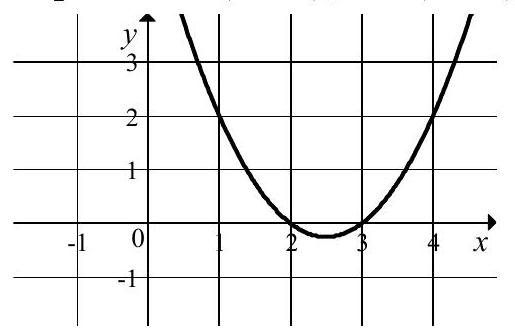
\includegraphics[max width=\textwidth, center]{2025_02_07_e6ecae3ec2e1f4241fbeg-06}
\end{itemize}

II sposób rozwiązania (realizacja pierwszego etapu)\\
Wyznaczamy postać kanoniczną trójmianu kwadratowego $x^{2}-5 x+6$ i zapisujemy nierówność w postaci, np. $\left(x-\frac{5}{2}\right)^{2}-\frac{1}{4}>0$, a następnie

\begin{itemize}
  \item przekształcamy nierówność tak, aby jej lewa strona była zapisana w postaci iloczynowej\\
$\left[\left(x-\frac{5}{2}\right)-\frac{1}{2}\right] \cdot\left[\left(x-\frac{5}{2}\right)+\frac{1}{2}\right]>0$,\\
$\left(x-\frac{6}{2}\right)\left(x-\frac{4}{2}\right)>0$,\\
albo
  \item przekształcamy nierówność do postaci równoważnej, korzystając z własności wartości bezwzględnej
\end{itemize}

$$
\left(x-\frac{5}{2}\right)^{2}>\frac{1}{4}
$$

$$
\left|x-\frac{5}{2}\right|>\frac{1}{2}
$$

Drugi etap rozwiązania:\\
Podajemy zbiór rozwiązań nierówności: $(-\infty, 2) \cup(3,+\infty)$ lub $x \in(-\infty, 2) \cup(3,+\infty)$.

\section*{Schemat oceniania Zdający otrzymuje}
 1 p. gdy:\begin{itemize}
  \item zrealizuje pierwszy etap rozwiązania i na tym poprzestanie lub błędnie zapisze zbiór rozwiązań nierówności, np.
  \item obliczy lub poda pierwiastki trójmianu kwadratowego $x_{1}=2, x_{2}=3$ i na tym poprzestanie lub błędnie zapisze zbiór rozwiązań nierówności,
  \item zaznaczy na wykresie miejsca zerowe funkcji $f(x)=x^{2}-5 x+6$ i na tym poprzestanie lub błędnie zapisze zbiór rozwiązań nierówności,
  \item rozłoży trójmian kwadratowy na czynniki liniowe, np. $(x-2)(x-3)$ i na tym poprzestanie lub błędnie zapisze zbiór rozwiązań nierówności,
  \item zapisze nierówność $\left|x-\frac{5}{2}\right|>\frac{1}{2}$ i na tym poprzestanie lub błędnie zapisze zbiór rozwiązań nierówności,\\
albo
  \item realizując pierwszy etap rozwiązania zadania popełni błąd (ale otrzyma dwa różne pierwiastki) i konsekwentnie do tego zapisze zbiór rozwiązań nierówności, np.
  \item popełni błąd rachunkowy przy obliczaniu wyróżnika lub pierwiastków trójmianu kwadratowego i konsekwentnie do popełnionego błędu zapisze zbiór rozwiązań nierówności,
  \item błędnie zapisze równania wynikające ze wzorów Viète'a, np.: $x_{1}+x_{2}=-\frac{5}{2}$ i konsekwentnie do popełnionego błędu zapisze zbiór rozwiązańn nierówności,
  \item błędnie zapisze nierówność, np. $\left|x+\frac{5}{2}\right|<\frac{1}{2}$ i konsekwentnie do popełnionego błędu zapisze zbiór rozwiązań nierówności.
\end{itemize}

\section*{Zdający otrzymuje}
gdy:

\begin{itemize}
  \item poda zbiór rozwiązań nierówności: $(-\infty, 2) \cup(3,+\infty)$ lub $x \in(-\infty, 2) \cup(3,+\infty)$ lub ( $x<2$ lub $x>3$ ),\\
albo
  \item sporządzi ilustrację geometryczną (oś liczbowa, wykres) i zapisze zbiór rozwiązań nierówności w postaci: $x<2, x>3$,\\
albo
  \item poda zbiór rozwiązań nierówności w postaci graficznej z poprawnie zaznaczonymi końcami przedziałów.
\end{itemize}

\section*{Uwagi}
\begin{enumerate}
  \item Jeżeli zdający dzieli obie strony nierówności przez $x-2$ bez stosownego założenia, to otrzymuje 0 punktów.
  \item Jeżeli zdający dzieli obie strony nierówności przez $x-2$, rozważając dwa przypadki $x-2>0$ oraz $x-2<0$, rozwiąże nierówność w każdym z tych przypadków, ale nie rozważy przypadku $x-2=0$, to otrzymuje 1 punkt.
\end{enumerate}

Kryteria uwzgledniajace specyficzne trudności w uczeniu sie matematyki

\begin{enumerate}
  \item Akceptujemy zapis przedziału nieuwzględniający porządku liczb na osi liczbowej, np.: $(2,-\infty)$.
  \item Jeżeli zdający poprawnie obliczy pierwiastki trójmianu $x_{1}=2, x_{2}=3$ i zapisze, np . $(-\infty,-2) \cup(3,+\infty)$, popełniając tym samym błąd przy przepisywaniu jednego z pierwiastków, to otrzymuje 2 punkty.
\end{enumerate}

\section*{Zadanie 27. (0-2)}
Wykaż, że dla dowolnej liczby rzeczywistej $x$ i dla dowolnej liczby rzeczywistej $y$ prawdziwa jest nierówność $4 x^{2}-8 x y+5 y^{2} \geq 0$.

\begin{verbatim}
V. Rozumowanie
i argumentacja.
\end{verbatim}

\begin{enumerate}
  \setcounter{enumi}{1}
  \item Wyrażenia algebraiczne. Zdający używa wzorów skróconego mnożenia na $(a \pm b)^{2}$ oraz $a^{2}-b^{2}$ (2.1).
\end{enumerate}

\section*{I sposób rozwiązania}
Nierówność $4 x^{2}-8 x y+5 y^{2} \geq 0$ przekształcamy w sposób równoważny

$$
\begin{aligned}
& y^{2}+4 x^{2}-8 x y+4 y^{2} \geq 0, \\
& y^{2}+(2 x-2 y)^{2} \geq 0
\end{aligned}
$$

Ta nierówność jest prawdziwa dla dowolnych liczb rzeczywistych $x$ i $y$, gdyż kwadrat każdej liczby jest nieujemny i suma kwadratów liczb nieujemnych również jest nieujemna.\\
To kończy dowód.\\
Schemat oceniania I sposobu rozwiązania\\
Zdający otrzymuje ........................................................................................................... 1 p.\\
gdy zapisze nierówność w postaci równoważnej $y^{2}+(2 x-2 y)^{2} \geq 0$ i na tym poprzestanie lub dalej popełnia błędy.\\
Zdający otrzymuje\\
gdy przeprowadzi pełny dowód.

\section*{II sposób rozwiązania}
Nierówność $4 x^{2}-8 x y+5 y^{2} \geq 0$ możemy potraktować jak nierówność kwadratową z niewiadomą $x$ lub - analogicznie - z niewiadomą $y$. Wyróżnik trójmianu stojącego po lewej stronie nierówności jest równy\\
$\Delta=(-8 y)^{2}-4 \cdot 4 \cdot\left(5 y^{2}\right)=-16 y^{2} \leq 0$.\\
Stąd i z faktu, że współczynnik przy $x^{2}$ trójmianu $f(x)=4 x^{2}-8 x y+5 y^{2}$ jest dodatni wynika, że trójmian ten przyjmuje tylko wartości nieujemne. To kończy dowód.

Schemat oceniania II sposobu Zdający otrzymuje\\
gdy wyznaczy wyróżnik trójmianu $f(x)=4 x^{2}-8 x y+5 y^{2}: \Delta=-16 y^{2}$ i na tym poprzestanie lub dalej popełnia błędy.

\section*{Zdajacy otrzymuje}
gdy wyznaczy wyróżnik trójmianu $f(x)=4 x^{2}-8 x y+5 y^{2}$, zapisze, że jest on niedodatni i wyciągnie wniosek, że trójmian przyjmuje tylko wartości nieujemne.

\section*{III sposób rozwiązania}
Dla dowolnych liczb rzeczywistych $x, y$ prawdziwa jest nierówność $x^{2}+y^{2} \geq 2 x y$. Stąd wynika, że prawdziwa jest nierówność

$$
4 x^{2}+4 y^{2} \geq 8 x y, \text { czyli } 4 x^{2}-8 x y+4 y^{2} \geq 0
$$

Zatem, dla dowolnych liczb $x, y$ mamy\\
$4 x^{2}-8 x y+5 y^{2} \geq 4 x^{2}-8 x y+4 y^{2} \geq 0$.\\
To kończy dowód.

\section*{Schemat oceniania III sposobu rozwiązania Zdajacy otrzymuje}
gdy zapisze, że dla dowolnych liczb rzeczywistych $x$, $y$ prawdziwe są nierówności $4 x^{2}-8 x y+5 y^{2} \geq 4 x^{2}-8 x y+4 y^{2}$ oraz $4 x^{2}+4 y^{2} \geq 8 x y$ (lub $x^{2}+y^{2} \geq 2 x y$ ).\\
Zdający otrzymuje\\
gdy przeprowadzi pełny dowód.

\section*{IV sposób rozwiązania}
Gdy co najmniej jedna $z$ liczb $x, y$ jest równa 0 , to nierówność $4 x^{2}-8 x y+5 y^{2} \geq 0$ jest prawdziwa, gdyż suma trzech liczb, z których co najmniej dwie są równe 0 , a trzecia nieujemna, jest nieujemna.\\
Gdy liczby $x, y$ są przeciwnych znaków, to $x y<0$, więc $-8 x y>0$. Zatem nierówność $4 x^{2}-8 x y+5 y^{2} \geq 0$ jest prawdziwa, gdyż lewa jej strona jest sumą trzech liczb dodatnich.\\
Pozostaje wykazać prawdziwość nierówności w przypadku, gdy liczby $x, y$ są tego samego znaku.\\
Zauważmy najpierw, że dla dowolnych liczb rzeczywistych $x, y$ prawdziwa jest nierówność $(2 x-\sqrt{5} y)^{2} \geq 0$, czyli $4 x^{2}-4 \sqrt{5} x y+5 y^{2} \geq 0$.

Wykażemy teraz prawdziwość nierówności

$$
4 x^{2}-8 x y+5 y^{2} \geq 4 x^{2}-4 \sqrt{5} x y+5 y^{2}
$$

równoważnie\\
$-8 x y \geq-4 \sqrt{5} x y$,\\
$x y \leq \frac{\sqrt{5}}{2} x y$.\\
Skoro $x$ i $y$ są tego samego znaku, to $x y>0$, więc dzieląc obie strony nierówności przez $x y$, otrzymujemy nierówność równoważną $1 \leq \frac{\sqrt{5}}{2}$, co jest prawdą. To kończy dowód.

\section*{Schemat oceniania IV sposobu rozwiązania \\
 Zdający otrzymuje 1 p.}
 gdy wykaże prawdziwość nierówności w przypadku, gdy co najmniej jedna z liczb $x, y$ jest równa 0 oraz w przypadku, gdy liczby $x, y$ są przeciwnych znaków, a w przypadku, gdy $x, y$ są tego samego znaku zauważy, że prawdziwa jest nierówność $(2 x-\sqrt{5} y)^{2} \geq 0$.Zdający otrzymuje\\
gdy przeprowadzi pełny dowód.

\section*{Uwaga}
Gdy zdający sprawdza jedynie prawdziwość nierówności dla konkretnych liczb $x$ i $y$, to otrzymuje 0 punktów.

\section*{Zadanie 28. (0-2)}
Dany jest kwadrat $A B C D$. Przekątne $A C$ i $B D$ przecinają się w punkcie $E$. Punkty $K$ i $M$ są środkami odcinków - odpowiednio - $A E$ i $E C$. Punkty $L$ i $N$ leżą na przekątnej $B D$ tak, że $|B L|=\frac{1}{3}|B E|$ i $|D N|=\frac{1}{3}|D E|$ (zobacz rysunek). Wykaż, że stosunek pola czworokąta KLMN do pola kwadratu $A B C D$ jest równy 1:3.\\
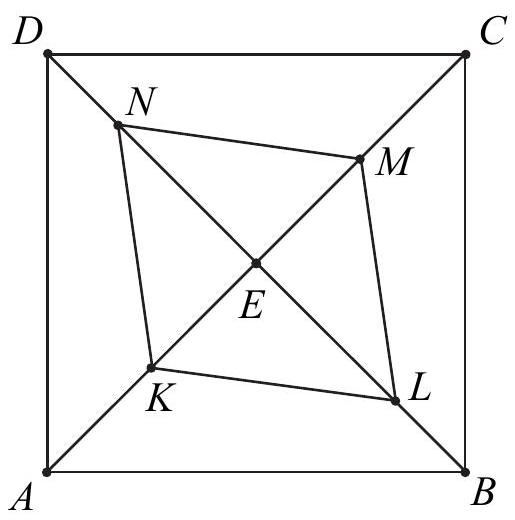
\includegraphics[max width=\textwidth, center]{2025_02_07_e6ecae3ec2e1f4241fbeg-10(1)}\\
V. Rozumowanie i argumentacja.

G10. Figury płaskie. Zdający oblicza pola i obwody trójkątów i czworokątów. (G10.9).

\section*{I sposób rozwiązania}
\begin{center}
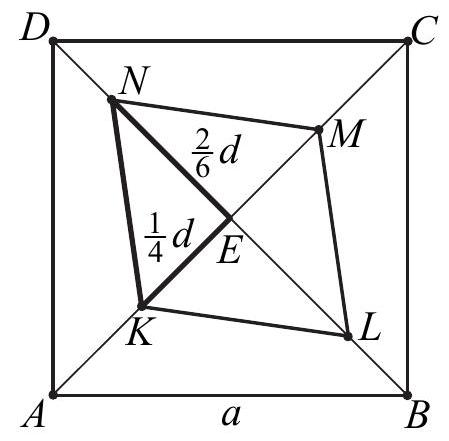
\includegraphics[max width=\textwidth]{2025_02_07_e6ecae3ec2e1f4241fbeg-10}
\end{center}

Przekątne w kwadracie $A B C D$ są równe, więc $|A C|=|B D|=d=a \sqrt{2}$.\\
Pole kwadratu $A B C D$ jest równe $P_{A B C D}=a^{2}$. Czworokąt $K L M N$ składa się z czterech trójkątów prostokątnych przystających do trójkąta $K E N$. Pole każdego z nich jest równe $P=\frac{1}{2} \cdot\left(\frac{1}{4} d\right) \cdot\left(\frac{2}{6} d\right)=\frac{1}{24} d^{2}=\frac{1}{24}(a \sqrt{2})^{2}=\frac{1}{24} \cdot 2 a^{2}=\frac{1}{12} a^{2}$.

Zatem pole czworokąta $K L M N$ jest równe

$$
P_{K L M N}=4 \cdot \frac{1}{12} a^{2}=\frac{1}{3} a^{2} .
$$

Stąd\\
$\frac{P_{K L M N}}{P_{A B C D}}=\frac{\frac{1}{3} a^{2}}{a^{2}}=\frac{1}{3}$.

\section*{II sposób rozwiązania}
\begin{center}
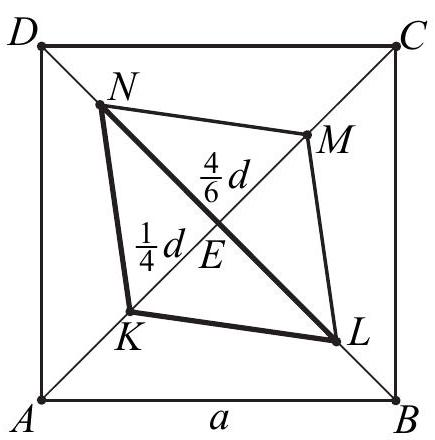
\includegraphics[max width=\textwidth]{2025_02_07_e6ecae3ec2e1f4241fbeg-11(1)}
\end{center}

Przekątne w kwadracie $A B C D$ są równe, więc $|A C|=|B D|=d=a \sqrt{2}$.\\
Pole kwadratu $A B C D$ jest równe $P_{A B C D}=a^{2}$. Czworokąt $K L M N$ składa się z dwóch trójkątów przystających do trójkąta $K L N$. Pole każdego z nich jest równe\\
$P=\frac{1}{2} \cdot\left(\frac{4}{6} d\right) \cdot\left(\frac{1}{4} d\right)=\frac{1}{12} d^{2}=\frac{1}{12}(a \sqrt{2})^{2}=\frac{1}{12} \cdot 2 a^{2}=\frac{1}{6} a^{2}$.\\
Zatem pole czworokąta $K L M N$ jest równe\\
$P_{K L M N}=2 \cdot \frac{1}{6} a^{2}=\frac{1}{3} a^{2}$.\\
Stąd\\
$\frac{P_{K L M N}}{P_{A B C D}}=\frac{\frac{1}{3} a^{2}}{a^{2}}=\frac{1}{3}$.

\section*{III sposób rozwiązania}
\begin{center}
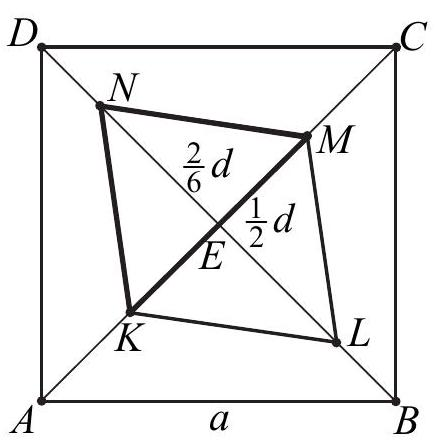
\includegraphics[max width=\textwidth]{2025_02_07_e6ecae3ec2e1f4241fbeg-11}
\end{center}

Przekątne w kwadracie $A B C D$ są równe, więc $|A C|=|B D|=d=a \sqrt{2}$.

Pole kwadratu $A B C D$ jest równe $P_{A B C D}=a^{2}$. Czworokąt $K L M N$ składa się z dwóch trójkątów przystających do trójkąta $K M N$. Pole każdego z nich jest równe\\
$P=\frac{1}{2} \cdot\left(\frac{1}{2} d\right) \cdot\left(\frac{2}{6} d\right)=\frac{1}{12} d^{2}=\frac{1}{12}(a \sqrt{2})^{2}=\frac{1}{12} \cdot 2 a^{2}=\frac{1}{6} a^{2}$.\\
Zatem pole czworokąta $K L M N$ jest równe\\
$P_{K L M N}=2 \cdot \frac{1}{6} a^{2}=\frac{1}{3} a^{2}$.\\
Stąd\\
$\frac{P_{K L M N}}{P_{A B C D}}=\frac{\frac{1}{3} a^{2}}{a^{2}}=\frac{1}{3}$.

\section*{IV sposób rozwiązania}
\begin{center}
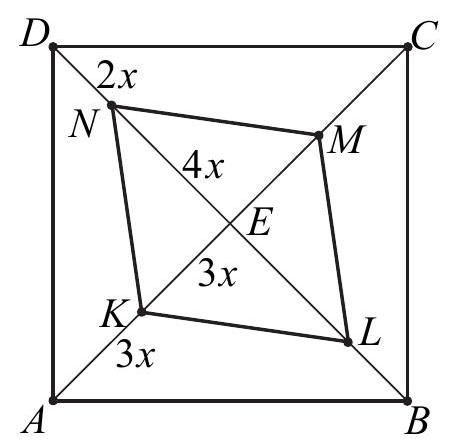
\includegraphics[max width=\textwidth]{2025_02_07_e6ecae3ec2e1f4241fbeg-12}
\end{center}

Ponieważ przekątne w kwadracie są równe, więc $|A E|=|E D|$. Niech $|A E|=|E D|=6 x$.\\
Wtedy\\
$|A K|=|K E|=|E M|=|M C|=3 x,|D N|=|L B|=2 x$ oraz $|N E|=|E L|=4 x$.\\
Stąd\\
$|K M|=|K E|+|E M|=6 x$ oraz $|N L|=|N E|+|E L|=8 x$.\\
Pole kwadratu $A B C D$ jest równe\\
$P_{A B C D}=\frac{1}{2}|A C| \cdot|B D|=\frac{1}{2} \cdot 12 x \cdot 12 x=72 x^{2}$.\\
Pole czworokąta $K L M N$ jest równe\\
$P_{K L M N}=\frac{1}{2}|K M| \cdot|N L|=\frac{1}{2} \cdot 6 x \cdot 8 x=24 x^{2}$.\\
Stąd\\
$\frac{P_{K L M N}}{P_{A B C D}}=\frac{24 x^{2}}{72 x^{2}}=\frac{1}{3}$.

\section*{Schemat oceniania}
\section*{Zdający otrzymuje}
\begin{itemize}
  \item gdy wyznaczy pole jednego z trójkątów: $K L E, L M E, M N E, N K E\left(P=\frac{1}{12} a^{2}\right)$\\
albo
  \item gdy wyznaczy pole jednego z trójkątów: $\operatorname{NLM}, \operatorname{LNK}\left(P=\frac{1}{6} a^{2}\right)$\\
albo
  \item gdy wyznaczy pole jednego z trójkątów: $K M N, K L M\left(P=\frac{1}{6} a^{2}\right)$\\
albo
  \item gdy wyznaczy pole czworokąta $K L M N$ w zależności od jego przekątnych, np.
\end{itemize}

$$
P_{K L M N}=\frac{1}{2}|K M| \cdot|L N|=\frac{1}{2} \cdot 6 x \cdot 8 x=24 x^{2}
$$

i na tym poprzestanie lub dalej popełnia błędy.

\section*{Zdający otrzymuje}
gdy wykaże, że $\frac{P_{K L M N}}{P_{A B C D}}=\frac{1}{3}$.

\section*{Uwagi}
\begin{enumerate}
  \item Jeżeli zdający przy wyznaczaniu pola kwadratu i pola czworokąta KLMN przyjmuje konkretne wartości liczbowe bez stosownego komentarza i rozwiązuje zadanie do końca, to otrzymuje 1 punkt.
  \item Jeżeli zdający przy wyznaczaniu pól trójkątów lub pól czworokątów o prostopadłych przekątnych pomija współczynnik $\frac{1}{2}$, otrzymując poprawny stosunek pola czworokąta $K L M N$ do pola kwadratu $A B C D$, to otrzymuje 1 punkt.
  \item Jeżeli zdający w swoim rozumowaniu wykorzystuje tezę, to za całe rozwiązanie otrzymuje 0 punktów.
\end{enumerate}

\section*{Zadanie 29. (0-2)}
Oblicz najmniejszą i największą wartość funkcji kwadratowej $f(x)=x^{2}-6 x+3$ w przedziale $\langle 0,4\rangle$.\\
II. Wykorzystanie\\
i interpretowanie reprezentacji.\\
4. Funkcje. Zdający wyznacza wartość najmniejszą i wartość największą funkcji kwadratowej w przedziale domkniętym (4.11).

\section*{Rozwiązanie}
Obliczamy pierwszą współrzędną wierzchołka paraboli o równaniu $y=x^{2}-6 x+3$ : $x_{w}=\frac{6}{2}=3$. Argument $x_{w}=3$ należy do przedziału $\langle 0,4\rangle$, więc najmniejszą wartością funkcji $f$ w przedziale $\langle 0,4\rangle$ jest $f(3)=-6$. Obliczamy wartości funkcji $f$ na końcach przedziału $\langle 0,4\rangle$ :\\
$f(0)=3$ oraz $f(4)=-5$.\\
Największą wartością jaką przyjmuje funkcja $f \mathrm{w}$ przedziale $\langle 0,4\rangle$ jest $f(0)=3$.

\section*{Schemat oceniania}
Zdający otrzymuje\\
gdy

\begin{itemize}
  \item obliczy pierwszą współłzędną wierzchołka paraboli $x_{w}=3$ i stwierdzi, że $x_{w} \in\langle 0,4\rangle$, albo
  \item obliczy wartości funkcji $f$ na końcach przedziału $\langle 0,4\rangle: f(0)=3$ oraz $f(4)=-5$.
\end{itemize}

Zdający otrzymuje 2 p. gdy zapisze odpowiedź: najmniejsza wartość funkcji $f \mathrm{w}$ przedziale $\langle 0,4\rangle$ jest równa $f(3)=-6$, a największa wartość funkcji w tym przedziale jest równa $f(0)=3$.

\section*{Uwagi}
\begin{enumerate}
  \item Jeżeli zdający obliczy jedynie trzy wartości funkcji: $f(0)=3, f(3)=-6$ i $f(4)=-5$ oraz sformułuje odpowiedź: największa wartość funkcji w przedziale $\langle 0,4\rangle$ jest równa 3, a najmniejsza wartość funkcji jest równa -6 , to otrzymuje 2 punkty.
  \item Jeżeli zdający obliczy tylko współrzędne wierzchołka paraboli $x_{w}=3, f(3)=-6$, ale nie zapisze, że $x_{w} \in\langle 0,4\rangle$, to otrzymuje $\mathbf{0}$ punktów.
\end{enumerate}

Zadanie 30. (0-2)\\
W układzie współrzędnych są dane punkty $A=(-43,-12), B=(50,19)$. Prosta $A B$ przecina oś $O x$ w punkcie $P$. Oblicz pierwszą wspórłzędną punktu $P$.\\
II. Wykorzystanie i interpretowanie reprezentacji.\\
3. Równania i nierówności. Zdający wyznacza równanie prostej przechodzącej przez dwa dane punkty. (8.1).

\section*{I sposób rozwiązania}
Wyznaczamy równanie prostej $A B$\\
$y=\frac{1}{3} x+\frac{7}{3}$ lub $x-3 y+7=0$.\\
Pierwsza współrzędna punktu $P$ jest miejscem zerowym funkcji liniowej określonej wzorem $y=\frac{1}{3} x+\frac{7}{3}$.\\
Rozwiązujemy zatem równanie\\
$\frac{1}{3} x+\frac{7}{3}=0$.\\
Stąd $x=-7$.\\
Schemat oceniania I sposobu rozwiązania\\
Zdający otrzymuje ........................................................................................................... 1 p.\\
gdy wyznaczy równanie prostej $A B$, np. w postaci $y=\frac{1}{3} x+\frac{7}{3}$ i na tym poprzestanie lub dalej popełnia błędy.\\
Zdający otrzymuje 2 p.\\
gdy obliczy pierwszą współrzędną punktu $P: x=-7$.

\section*{Uwagi}
\begin{enumerate}
  \item Jeżeli zdający przy wyznaczaniu równania prostej $A B$, popełni błąd rzeczowy, to otrzymuje 0 punktów.
  \item Jeżeli zdający wyznaczy równanie prostej $A B$, popełniając błędy rachunkowe (np. zapisze $(19-12)(x-50)-(50-43)(y-19)=0)$ i konsekwentnie obliczy pierwszą współrzędną punktu $P$, to otrzymuje 1 punkt.
\end{enumerate}

\section*{II sposób rozwiązania}
Niech $P=(p, 0)$ będzie punktem przecięcia prostej $A B$ z osią $O x$ układu współrzędnych, a punkty $C$ i $D$ będą rzutami prostokątnymi punktów odpowiednio $A$ i $B$ na tę oś.\\
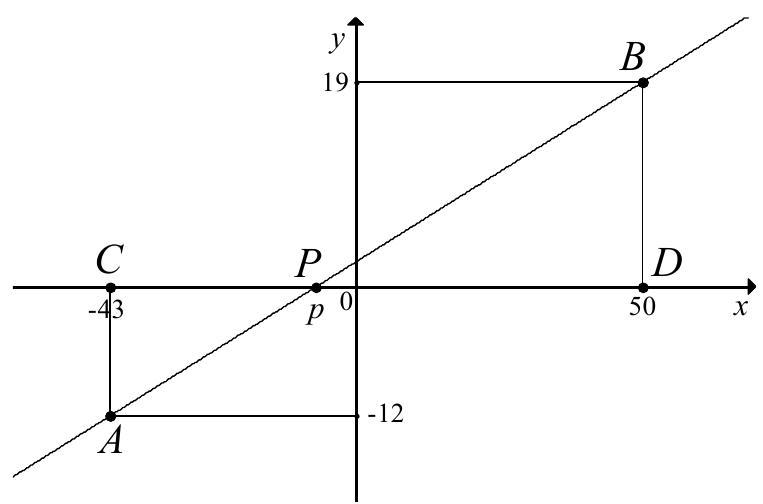
\includegraphics[max width=\textwidth, center]{2025_02_07_e6ecae3ec2e1f4241fbeg-16}

Wtedy $C=(-43,0)$ i $D=(50,0)$. Trójkąty $P A C$ i $P B D$ są podobne (oba są prostokątne, a ich kąty ostre przy wierzchołku $P$ są równe). Zatem\\
$\frac{|P D|}{|B D|}=\frac{|P C|}{|A C|}$, czyli $\frac{50-p}{19}=\frac{p-(-43)}{12}$.\\
Stąd\\
$12(50-p)=19(p+43)$,\\
$600-12 p=19 p+817$,\\
$-31 p=217$,\\
$p=-7$.\\
Schemat oceniania II sposobu rozwiązania\\
Zdający otrzymuje\\
gdy zapisze równanie, w którym niewiadomą jest pierwsza współrzędna punktu $P, \mathrm{np}$.:\\
$\frac{50-p}{19}=\frac{p-(-43)}{12}$ i na tym poprzestanie lub dalej popełnia błędy.\\
Zdający otrzymuje\\
2 p.\\
gdy obliczy pierwszą współrzędną punktu $P: p=-7$.

Kryteria uwzgledniajace specyficzne trudności w uczeniu sie matematyki\\
Jeżeli zdający obliczy pierwszą współrzędną punktu $P$, zapisując np. $x=-7$, ale popełni błąd formułując odpowiedź, np. $P=(7,0), P=(0,-7)$, to otrzymuje 2 punkty.

\section*{Zadanie 31. (0-2)}
Jeżeli do licznika i do mianownika nieskracalnego dodatniego ułamka dodamy połowę jego licznika, to otrzymamy $\frac{4}{7}$, a jeżeli do licznika i do mianownika dodamy 1 , to otrzymamy $\frac{1}{2}$. Wyznacz ten ułamek.

\begin{center}
\begin{tabular}{|c|l}
\hline
\begin{tabular}{c}
III. Modelowanie \\
matematyczne. \\
\end{tabular} & \begin{tabular}{l}
G7. Równania. Zdający za pomoca równań lub układów \\
równań opisuje i rozwiązuje zadania osadzone w kontekście \\
praktycznym, a także rozwiązuje układy równań stopnia \\
pierwszego z dwiema niewiadomymi (G7.7, G7.6). \\
\end{tabular} \\
\hline
\end{tabular}
\end{center}

\section*{I sposób rozwiązania}
Niech $x$ i $y$ oznaczają odpowiednio licznik i mianownik szukanego ułamka nieskracalnego. Z treści zadania otrzymujemy układ równań\\
$\frac{x+\frac{1}{2} x}{y+\frac{1}{2} x}=\frac{4}{7}$ oraz $\frac{x+1}{y+1}=\frac{1}{2}$,\\
$7 \cdot \frac{3}{2} x=4\left(y+\frac{1}{2} x\right)$ oraz $2(x+1)=y+1$,\\
$\frac{21}{2} x=4 y+2 x$ oraz $2 x+1=y$.\\
Stąd\\
$\frac{17}{2} x=4(2 x+1)$,\\
$17 x=16 x+8$,\\
$x=8$, więc $y=2 \cdot 8+1=17$.\\
Zatem szukany ułamek to $\frac{8}{17}$. Jest to ułamek nieskracalny.

\section*{Schemat oceniania I sposobu rozwiązania \\
 Zdający otrzymuje}
1 p.\\
gdy

\begin{itemize}
  \item zapisze układ równań z dwiema niewiadomymi, np.: $\frac{x+\frac{1}{2} x}{y+\frac{1}{2} x}=\frac{4}{7} \mathrm{i} \frac{x+1}{y+1}=\frac{1}{2}$\\
albo
  \item zapisze równanie z jedną niewiadomą, $\mathrm{np} .: \frac{17}{2} x=4(2 x+1)$.
\end{itemize}

\section*{Zdający otrzymuje}
gdy wyznaczy szukany ułamek: $\frac{8}{17}$.

\section*{II sposób rozwiązania}
Niech $x$ i $y$ oznaczają odpowiednio licznik i mianownik szukanego ułamka nieskracalnego. $Z$ treści zadania otrzymujemy równanie\\
$\frac{x+\frac{1}{2} x}{y+\frac{1}{2} x}=\frac{4}{7}$,\\
$\frac{\frac{3}{2} x}{y+\frac{1}{2} x}=\frac{4}{7}$,\\
$\frac{21}{2} x=4 y+2 x$,\\
$\frac{17}{2} x=4 y$.\\
Stąd\\
$\frac{x}{y}=\frac{8}{17}$.\\
Otrzymany ułamek jest nieskracalny oraz $\frac{x+1}{y+1}=\frac{9}{18}=\frac{1}{2}$.\\
Stąd wynika, że $\frac{8}{17}$ to jedyny szukany ułamek.\\
Schemat oceniania II sposobu rozwiązania Zdający otrzymuje\\
gdy zapisze równanie z dwiema niewiadomymi: $\frac{x+\frac{1}{2} x}{y+\frac{1}{2} x}=\frac{4}{7}$ i doprowadzi je postaci $\frac{x}{y}=\frac{8}{17}$ i na tym zakończy\\
Zdający otrzymuje\\
gdy zapisze równanie z dwiema niewiadomymi: $\frac{x+\frac{1}{2} x}{y+\frac{1}{2} x}=\frac{4}{7}$, doprowadzi je postaci $\frac{x}{y}=\frac{8}{17}$\\
i sprawdzi, że ułamek ten spełnia drugi $z$ warunków podanych $w$ treści zadania: $\frac{x+1}{y+1}=\frac{9}{18}=\frac{1}{2}$.

\section*{Uwagi:}
\begin{enumerate}
  \item Jeżeli zdający od razu poda ułamek $\frac{8}{17}$ i nie sprawdzi, że $\frac{8+1}{17+1}=\frac{1}{2}$, to otrzymuje 0 punktów.
  \item Jeżeli zdający od razu poda ułamek $\frac{8}{17}$ i sprawdzi, że spełnia on drugi z warunków podanych w treści zadania $\frac{8+1}{17+1}=\frac{1}{2}$, to otrzymuje $\mathbf{1}$ punkt.
\end{enumerate}

Zadanie 32. (0-4)\\
Wysokość graniastosłupa prawidłowego czworokątnego jest równa 16. Przekątna graniastosłupa jest nachylona do płaszczyzny jego podstawy pod kątem, którego cosinus jest równy $\frac{3}{5}$. Oblicz pole powierzchni całkowitej tego graniastosłupa.

\section*{IV. Użycie i tworzenie strategii.}
\begin{enumerate}
  \setcounter{enumi}{8}
  \item Stereometria. Zdający stosuje trygonometrię do obliczeń długości odcinków, miar kątów, pól powierzchni i objętości (9.6).
\end{enumerate}

\section*{I sposób rozwiązania}
Niech $a$ oznacza długość krawędzi podstawy tego graniastosłupa i niech $\alpha$ będzie kątem nachylenia przekątnej graniastosłupa do płaszczyzny jego podstawy (zobacz rysunek).\\
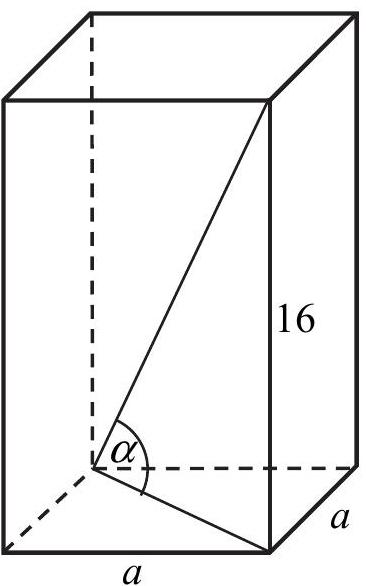
\includegraphics[max width=\textwidth, center]{2025_02_07_e6ecae3ec2e1f4241fbeg-19}

Ponieważ $\cos \alpha=\frac{3}{5}$, więc kąt $\alpha$ jest ostry oraz $\sin \alpha=\frac{4}{5}$. Stąd wynika, że $\operatorname{tg} \alpha=\frac{4}{3}$. Z drugiej strony $\operatorname{tg} \alpha=\frac{16}{a \sqrt{2}}$. Obliczamy długość krawędzi podstawy graniastosłupa.\\
Rozwiązujemy równanie:\\
$\frac{16}{a \sqrt{2}}=\frac{4}{3}$, skąd $a=6 \sqrt{2}$.\\
Szukane pole powierzchni całkowitej tego graniastosłupa jest równe:\\
$P_{c}=2 \cdot(6 \sqrt{2})^{2}+4 \cdot 6 \sqrt{2} \cdot 16=144+384 \sqrt{2}=48(3+8 \sqrt{2})$.

\section*{II sposób rozwiązania}
Niech $a$ oznacza długość krawędzi podstawy tego graniastosłupa, $\alpha$ - kąt nachylenia przekątnej graniastosłupa do płaszczyzny jego podstawy oraz niech przekątna podstawy graniastosłupa ma długość $3 x$, a przekątna graniastosłupa $5 x$ (zobacz rysunek).\\
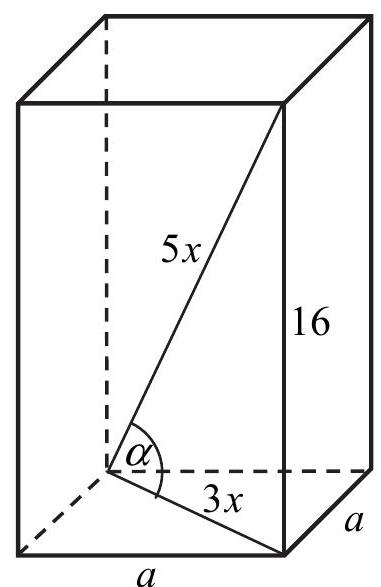
\includegraphics[max width=\textwidth, center]{2025_02_07_e6ecae3ec2e1f4241fbeg-20}

Z twierdzenia Pitagorasa otrzymujemy równanie\\
$(3 x)^{2}+16^{2}=(5 x)^{2}$,\\
$9 x^{2}+256=25 x^{2}$,\\
$256=16 x^{2}$,\\
$16=x^{2}$.\\
Stąd $x=4$. Zatem przekątna podstawy graniastosłupa ma długość $3 x=3 \cdot 4=12$.\\
Obliczamy długość krawędzi podstawy graniastosłupa:\\
$a \sqrt{2}=12$, skąd $a=6 \sqrt{2}$.\\
Szukane pole powierzchni całkowitej tego graniastosłupa jest równe:\\
$P_{c}=2 \cdot(6 \sqrt{2})^{2}+4 \cdot 6 \sqrt{2} \cdot 16=144+384 \sqrt{2}=48(3+8 \sqrt{2})$.

\section*{Uwaga}
Możemy również zauważyć, że trójkąt prostokątny o kącie ostrym $\alpha$ takim, że $\cos \alpha=\frac{3}{5}$ jest podobny do trójkąta pitagorejskiego o bokach długości 3, 4 i 5. Skala tego podobieństwa jest równa $x=\frac{16}{4}=4$. W rezultacie szukane pole $P_{c}$ powierzchni całkowitej graniastosłupa jest równe $x^{2} P_{m}$, gdzie $P_{m}$ to pole powierzchni całkowitej graniastosłupa, którego przekątna ma długość 5, a przekątna podstawy długość 3 . Długość krawędzi podstawy tego graniastosłupa jest równa $\frac{3}{\sqrt{2}}=\frac{3}{2} \sqrt{2}$, więc $P_{m}=2 \cdot\left(\frac{3}{2} \sqrt{2}\right)^{2}+4 \cdot \frac{3}{2} \sqrt{2} \cdot 4=9+24 \sqrt{2}$.\\
Zatem $P_{c}=4^{2} \cdot P_{m}=16(9+24 \sqrt{2})=48(3+8 \sqrt{2})$.

\section*{Schemat oceniania I i II sposobu rozwiązania}
Rozwiązanie, w którym postęp jest niewielki, ale konieczny na drodze do pełnego rozwiązania.\\
Zdający:

\begin{itemize}
  \item zapisze, że $\operatorname{tg} \alpha=\frac{4}{3}$\\
albo
  \item zapisze równanie, z którego można obliczyć skalę $x$ podobieństwa trójkąta o bokach długości 3, 4 i 5 do trójkąta o przyprostokątnej długości 16 leżącej naprzecio kąta $\alpha$, np. $(3 x)^{2}+16^{2}=(5 x)^{2}$\\
albo
  \item poda skalę $x$ podobieństwa trójkąta o bokach długości 3, 4 i 5 do trójkąta o przyprostokątnej długości 16 leżącej naprzeciw kąta $\alpha, x=4$\\
albo
  \item zaznaczy na rysunku kąt nachylenia przekątnej graniastosłupa do płaszczyzny jego podstawy\\
albo
  \item zapisze, że długość $d$ przekątnej graniastosłupa jest równa 20 i na tym zakończy lub dalej popełni błędy.
\end{itemize}

\section*{Rozwiązanie, w którym jest istotny postęp \\
 Zdający:}
\begin{itemize}
  \item obliczy długość e przekątnej podstawy tego graniastosłupa $e=12$\\
albo
  \item zapisze równanie, z którego można obliczyć długość krawędzi podstawy tego graniastosłupa, np. $16^{2}+(a \sqrt{2})^{2}=\left(\frac{5 a \sqrt{2}}{3}\right)^{2}$\\
$16^{2}+(a \sqrt{2})^{2}=20^{2}$ lub $\frac{16}{a \sqrt{2}}=\frac{4}{3}$\\
albo
  \item zapisze układ równań, z którego można obliczyć długość krawędzi podstawy tego graniastosłupa, np.\\
$\left\{\begin{array}{l}\frac{a \sqrt{2}}{d}=\frac{3}{5} \\ (a \sqrt{2})^{2}+16^{2}=d^{2}\end{array}\right.$\\
gdzie $d$ oznacza długość przekątnej tego graniastosłupa\\
i na tym zakończy lub dalej popełni błędy.
\end{itemize}

\section*{Pokonanie zasadniczych trudności zadania}
Zdający obliczy długość krawędzi podstawy graniastosłupa: $a=6 \sqrt{2}$ i na tym zakończy lub dalej popełni błędy.

\section*{Rozwiązanie pelne}
Zdający obliczy pole powierzchni całkowitej tego graniastosłupa: $P_{c}=48(3+8 \sqrt{2})$.

\section*{Uwagi}
\begin{enumerate}
  \item Akceptujemy sytuację, w której zdający wprowadza do rozwiązania poprawne przybliżenia dziesiętne liczb rzeczywistych.
  \item Jeżeli zdający przyjmie miarę kąta nachylenia, która nie wynika z treści zadania (np. $\alpha=30^{\circ}$ ), i w rozwiązaniu z tego korzysta, to za całe rozwiązanie otrzymuje $\mathbf{0}$ punktów.
  \item Jeżeli zdający błędnie zaznaczy na rysunku podany kąt i korzysta $z$ tego kąta, to za całe rozwiązanie otrzymuje 0 punktów.
  \item Jeżeli zdający zapisze, że $\sin \alpha=\frac{3}{5}$ i korzysta z tej równości, to za całe rozwiązanie może otrzymać co najwyżej $\mathbf{1}$ punkt.
  \item Jeżeli zdający zapisze błędnie, że $e=a \sqrt{3}$, to za całe rozwiązanie może otrzymać co najwyżej 2 punkty.
\end{enumerate}

\section*{Zadanie 33. (0-4)}
Wśród 115 osób przeprowadzono badania ankietowe, związane z zakupami w pewnym kiosku. W poniższej tabeli przedstawiono informacje o tym, ile osób kupiło bilety tramwajowe ulgowe oraz ile osób kupiło bilety tramwajowe normalne.

\begin{center}
\begin{tabular}{|l|l|}
\hline
\begin{tabular}{l}
Rodzaj kupionych \\
biletów \\
\end{tabular} & Liczba osób \\
\hline
ulgowe & 76 \\
\hline
normalne & 41 \\
\hline
\end{tabular}
\end{center}

Uwaga! 27 osób spośród ankietowanych kupiło oba rodzaje biletów.\\
Oblicz prawdopodobieństwo zdarzenia polegającego na tym, że osoba losowo wybrana spośród ankietowanych nie kupiła żadnego biletu. Wynik przedstaw w formie nieskracalnego ułamka.

\begin{center}
\begin{tabular}{|c|l|}
\hline
\begin{tabular}{r}
III. Modelowanie \\
matematyczne. \\
\end{tabular} & \begin{tabular}{l}
10. Elementy statystyki opisowej. Teoria prawdopodobieństwa \\
i kombinatoryka. Zdajacy oblicza prawdopodobieństwa \\
w prostych sytuacjach, stosując klasyczną definicję \\
prawdopodobieństwa (10.3). \\
\end{tabular} \\
\hline
\end{tabular}
\end{center}

\section*{I sposób rozwiązania}
Oznaczmy:\\
$A$ - zdarzenie polegające na wylosowaniu osoby, która kupiła bilet ulgowy,\\
$B$ - zdarzenie polegające na wylosowaniu osoby, która kupiła bilet normalny,\\
$C$ - zdarzenie polegające na wylosowaniu osoby, która nie kupiła żadnego z wymienionych biletów.\\
Ankietę przeprowadzono wśród 115 osób, zatem $|\Omega|=115$.\\
Ponieważ wśród badanych występują osoby, które kupiły bilety obu rodzajów, więc\\
$|A \cup B|=|A|+|B|-|A \cap B|$.\\
Stąd $|A \cup B|=76+41-27=90$.\\
Zatem $|C|=|\Omega|-|A \cup B|=25$, więc\\
$P(C)=\frac{25}{115}=\frac{5}{23}$\\
Odp. Prawdopodobieństwo zdarzenia, polegającego na tym, że losowo wybrana spośród badanych osoba nie zakupiła żadnego z wymienionych biletów jest równe $\frac{5}{23}$.

\section*{II sposób rozwiązania}
Oznaczmy:\\
$C$ - zdarzenie polegające na wylosowaniu osoby, która nie kupiła żadnego biletu.\\
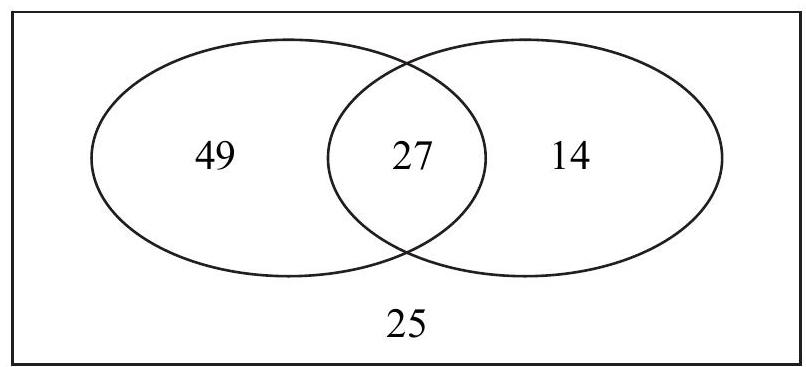
\includegraphics[max width=\textwidth, center]{2025_02_07_e6ecae3ec2e1f4241fbeg-23}

Liczba wszystkich zdarzeń elementarnych jest równa $|\Omega|=115$.\\
Liczba wszystkich osób, które kupiły co najmniej jeden bilet jest równa\\
$49+27+14=90$.\\
Zatem $|C|=115-90=25$.\\
Stąd $P(C)=\frac{25}{115}=\frac{5}{23}$.\\
Odp. Prawdopodobieństwo zdarzenia, polegającego na tym, że losowo wybrana spośród badanych osoba nie zakupiła żadnego z wymienionych biletów jest równe $\frac{5}{23}$.

\section*{Schemat oceniania I i II sposobu rozwiązania}
Rozwiązanie, w którym postęp jest niewielki, ale konieczny na drodze do pełnego rozwiązania 1 p. Zdający:

\begin{itemize}
  \item zapisze liczbę wszystkich zdarzeń elementarnych: $|\Omega|=115$\\
albo
  \item obliczy, ile jest wszystkich osób, które kupiły tylko bilety ulgowe: 49\\
albo
  \item obliczy, ile jest wszystkich osób, które kupiły tylko bilety normalne: 14\\
albo
  \item obliczy, ile jest wszystkich osób, które kupiły co najmniej jeden bilet: 90.
\end{itemize}

Rozwiązanie, w którym jest istotny postęp 2 p.\\
Zdający:

\begin{itemize}
  \item zapisze liczbę wszystkich zdarzeń elementarnych oraz obliczy, ile jest wszystkich osób, które kupiły tylko bilety ulgowe: $|\Omega|=115,49$\\
albo
  \item zapisze liczbę wszystkich zdarzeń elementarnych oraz obliczy, ile jest wszystkich osób, które kupiły tylko bilety normalne: $|\Omega|=115,14$\\
albo
  \item zapisze liczbę wszystkich zdarzeń elementarnych oraz obliczy, ile jest wszystkich osób, które kupiły co najmniej jeden bilet: $|\Omega|=115,90$\\
albo
  \item obliczy, ile jest wszystkich osób, które nie kupiły żadnego biletu: 25 .
\end{itemize}

\section*{Pokonanie zasadniczych trudności zadania}
Zdający zapisze liczbę wszystkich zdarzeń elementarnych oraz obliczy, ile jest wszystkich osób, które nie kupiły żadnego biletu: $|\Omega|=115,25$.\\
Rozwiązanie pelne\\
Zdający obliczy prawdopodobieństwo wylosowania osoby, która nie kupiła żadnego biletu i zapisze je w postaci ułamka nieskracalnego: $\frac{5}{23}$.

\section*{Uwagi}
\begin{enumerate}
  \item Jeśli zdający rozwiąże zadanie do końca i otrzyma $P(C)>1$ lub $P(C)<0$, to za całe rozwiązanie otrzymuje $\mathbf{0}$ punktów.
  \item Jeżeli zdający poda tylko wynik końcowy $P(C)=\frac{5}{23}$ lub $P(C)=\frac{25}{115}$, to otrzymuje $\mathbf{1}$ punkt.
  \item Jeżeli zdający obliczy $P(C)=\frac{25}{115}$ i nie przedstawi wyniku w postaci ułamka nieskracalnego, to otrzymuje 3 punkty.
  \item Jeżeli zdający popełni błąd rachunkowy przy wyznaczaniu $|A \cup B|$ lub $|C|$, i konsekwentnie do popełnionego błędu rozwiąże zadanie do końca, to otrzymuje co najwyżej $\mathbf{3}$ punkty.
  \item Jeżeli zdający sporządził diagram, na którym zapisał liczby 49, 27, 14 i 25,\\
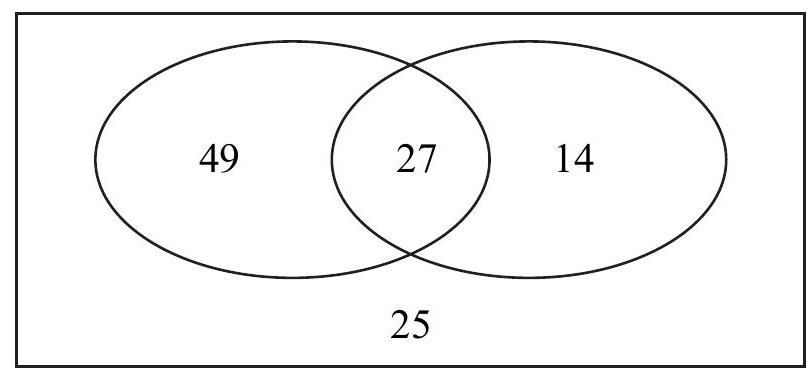
\includegraphics[max width=\textwidth, center]{2025_02_07_e6ecae3ec2e1f4241fbeg-24}\\
i na tym zakończyl, to otrzymuje 2 punkty.
\end{enumerate}

\section*{Zadanie 34. (0-5)}
W nieskończonym ciągu arytmetycznym $\left(a_{n}\right)$, określonym dla $n \geq 1$, suma jedenastu początkowych wyrazów tego ciągu jest równa 187. Średnia arytmetyczna pierwszego, trzeciego i dziewiątego wyrazu tego ciągu, jest równa 12 . Wyrazy $a_{1}, a_{3}, a_{k}$ ciągu $\left(a_{n}\right)$, w podanej kolejności, tworzą nowy ciąg - trzywyrazowy ciąg geometryczny $\left(b_{n}\right)$. Oblicz $k$.

\begin{center}
\begin{tabular}{|l|l|}
\hline
\begin{tabular}{c}
IV. Użycie i tworzenie \\
strategii. \\
\end{tabular} & \begin{tabular}{l}
5. Ciągi. Zdający stosuje wzór na $n$-ty wyraz i na sumę \\
$n$ początkowych wyrazów ciągu arytmetycznego stosuje wzór \\
na $n$-ty wyraz i na sumę $n$ początkowych wyrazów ciągu \\
geometrycznego (5.3, 5.4). \\
\end{tabular} \\
\hline
\end{tabular}
\end{center}

\section*{Rozwiązanie}
Korzystamy ze wzoru na sumę $n$ początkowych wyrazów ciągu arytmetycznego i zapisujemy równanie:\\
$\frac{2 a_{1}+10 r}{2} \cdot 11=187$,\\
$\left(a_{1}+5 r\right) \cdot 11=187$,\\
$a_{1}+5 r=17$.\\
Korzystamy z informacji o średniej arytmetycznej trzech wyrazów i zapisujemy równanie:\\
$\frac{a_{1}+a_{1}+2 r+a_{1}+8 r}{3}=12$,\\
$\frac{3 a_{1}+10 r}{3}=12$,\\
$a_{1}+\frac{10}{3} r=12$.\\
Zapisujemy układ równań:\\
$\left\{\begin{array}{l}a_{1}+5 r=17 \\ a_{1}+\frac{10}{3} r=12 .\end{array}\right.$\\
Z pierwszego równania otrzymujemy $a_{1}=17-5 r$.\\
Otrzymaną wartość $a_{1}$ podstawiamy do drugiego równania i otrzymujemy równanie z niewiadomą $r$ :\\
$17-5 r+\frac{10}{3} r=12$,\\
$r=3$.\\
Obliczamy pierwszy wyraz: $a_{1}=2$.

\section*{Uwaga}
W rozwiązaniu układu równań zdający może najpierw wyznaczyć niewiadomą $r=\frac{17}{5}-\frac{1}{5} a_{1}$. Otrzymaną wartość $r$ podstawiamy do drugiego równania i otrzymujemy równanie z niewiadomą $a_{1}$ :\\
$a_{1}+\frac{10}{3}\left(\frac{17}{5}-\frac{1}{5} a_{1}\right)=12$,\\
$a_{1}+\frac{170}{15}-\frac{10}{15} a_{1}=12$,\\
$\frac{1}{3} a_{1}=\frac{2}{3}$,\\
$a_{1}=2$.\\
Dla $a_{1}=2$ mamy $r=3$.\\
Wyznaczamy pozostałe wyrazy tworzące ciąg geometryczny:\\
$a_{3}=a_{1}+2 r=8, a_{k}=a_{1}+(k-1) r=2+(k-1) \cdot 3$.\\
Kolejne wyrazy $a_{1}, a_{3}, a_{k}$ ciągu geometrycznego spełniają warunek: $a_{3}{ }^{2}=a_{1} \cdot a_{k}$, stąd\\
$8^{2}=2 \cdot[2+(k-1) \cdot 3]$,\\
$32=3 k-1$,\\
$k=11$.\\
Dla $k=11$ wyrazy $a_{1}, a_{3}, a_{k}$ w podanej kolejności tworzą ciąg geometryczny.

\section*{Schemat oceniania}
Rozwiązanie, w którym postęp\\
Zdajaç wykorzysta

\begin{itemize}
  \item wzór na sumę n-początkowych wyrazów ciągu arytmetycznego i zapisze równanie z dwiema niewiadomymi $a_{1}$ i $r$, np.: $\frac{2 a_{1}+10 r}{2} \cdot 11=187$ lub $a_{1}+5 r=17$\\
albo
  \item średnią arytmetyczną pierwszego, trzeciego oraz dziewiątego wyrazu ciągu $\left(a_{n}\right)$ i zapisze równanie z dwiema niewiadomymi $a_{1} \mathrm{i} r$, np.:
\end{itemize}

$$
\frac{a_{1}+a_{1}+2 r+a_{1}+8 r}{3}=12 \text { lub } a_{1}+\frac{10}{3} r=12
$$

albo

\begin{itemize}
  \item zależność między pierwszym, trzecim i $k$-tym wyrazem ciągu $\left(a_{n}\right)$ wynikającą z faktu, że ciąg $\left(a_{1}, a_{3}, a_{k}\right)$ jest geometryczny i zapisze np.: $a_{3}{ }^{2}=a_{1} \cdot a_{k}$.
\end{itemize}

Rozwiązanie, w którym jest istotny postęp 2 p.\\
Zdający zapisze układ równań z dwiema niewiadomymi $a_{1} \mathrm{i} r$, np.: $\left\{\begin{array}{l}a_{1}+5 r=17 \\ a_{1}+\frac{10}{3} r=12\end{array}\right.$.\\
Pokonanie zasadniczych trudności zadania. 3 p.\\
Zdający rozwiąże układ równań $a_{1}=2$ i $r=3$ oraz zapisze zależność między pierwszym, trzecim i $k$-tym wyrazem ciągu $\left(a_{n}\right)$ wynikająca $z$ faktu, że ciąg $\left(a_{1}, a_{3}, a_{k}\right)$ jest geometryczny, np.: $a_{3}{ }^{2}=a_{1} \cdot a_{k}$.

\section*{Rozwiązanie zadania do końca, lecz z usterkami, które jednak nie przekreślają poprawności rozwiązania (np. błędy rachunkowe)}
\begin{itemize}
  \item zapisze równanie z niewiadomą $k$ wynikające z faktu, że ciąg $\left(a_{1}, a_{3}, a_{k}\right)$ jest geometryczny oraz $a_{k}$ jest $k$-tym wyrazem ciągu arytmetycznego, np.:
\end{itemize}

$$
8^{2}=2(2+(k-1) \cdot 3)
$$

albo

\begin{itemize}
  \item rozwiąże układ równań z błędem rachunkowym i konsekwentnie do popełnionego błędu obliczy $k$, o ile otrzymana wartość $k$ jest całkowita dodatnia.
\end{itemize}



\section*{Uwagi}
\begin{enumerate}
  \item Jeżeli zdający od razu poda $a_{1}=2$ i $r=3$ lub wypisze kolejne wyrazy ciągu arytmetycznego: $2,5,8,11, \ldots$, ale nie uzasadni, że jest to jedyny ciąg spełniający warunki zadania i na tym zakończy, to otrzymuje 1 punkt.
  \item Jeżeli zdający od razu poda $a_{1}=2$ i $r=3$ lub wypisze kolejne wyrazy ciągu arytmetycznego: $2,5,8,11, \ldots$, ale nie uzasadni, że jest to jedyny ciąg spełniający warunki zadania i wskaże lub obliczy $k=11$, to otrzymuje 3 punkty.
  \item Jeżeli zdający od razu poda $a_{1}=2$ i $r=3$ lub wypisze kolejne wyrazy ciągu arytmetycznego: $2,5,8,11, \ldots$, ale nie uzasadni, że jest to jedyny ciąg spełniający warunki zadania i zapisze równanie z niewiadomą $k$ i popełni błąd rachunkowy w trakcie jego rozwiązywania, to otrzymuje 2 punkty.
  \item Jeżeli zdający od razu przyjmie ciąg arytmetyczny nie spełniający warunków zadania (suma 11 początkowych jego wyrazów jest różna od 187 lub średnia pierwszego, trzeciego i dziewiątego wyrazu jest różna od 12), to za całe zadanie otrzymuje $\mathbf{0}$ punktów.
\end{enumerate}

\end{document}